
\subsubsection{\crossnextrow}

The idea this gadget is to assemble after reading the MSD, routing the counter back to the start of the
next row, in position for the counter to begin reading the first digit.

\vspace{.5cm}
For each $\inc\in \{ {\tt increment}, {\tt copy} \}$:

\begin{itemize}
    \item Create
    $\begin{aligned}[t]
        \crossnextrow(&\left\langle {\tt CrossNextRow},                   \inc \right\rangle,
                       \left\langle {\tt CounterRead},        1, \lambda, \inc \right\rangle \;)
    \end{aligned}$\\from the gadget shown in Figure~\ref{fig:cross_next_row}.
\end{itemize}
%
In this step, $6g + 4 \leq$
%
$6 \frac{d}{3} + 4 =$
%
$2d + 4 =$
%
$O\left( d \right) =$
%
$O\left( k \right) =$
%
$O\left( {\log N} \right)$ tiles were created.
%

\begin{figure}[H]
    \centering
    \subcaptionbox{
        General. There are $6g + 4$ tiles in this gadget.
        \label{fig:cross_next_row}
    }{\makebox[0.24\textwidth][c]{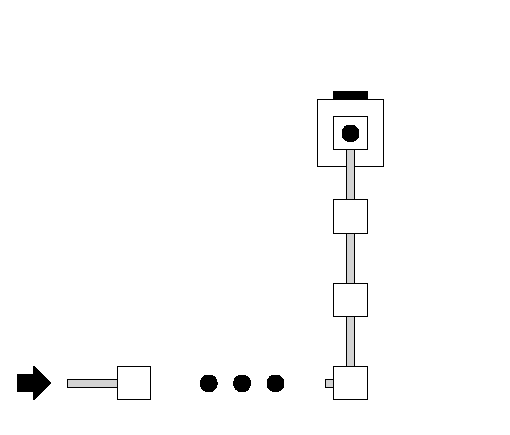
\includegraphics[width=1in]{cross_next_row}}}%
    ~
    \subcaptionbox{
        General overview.
        The black tiles in this figure is the gadget shown in subfigure~\subref{fig:cross_next_row}.
        \label{fig:cross_next_row_overview}
    }{\makebox[0.30\textwidth][c]{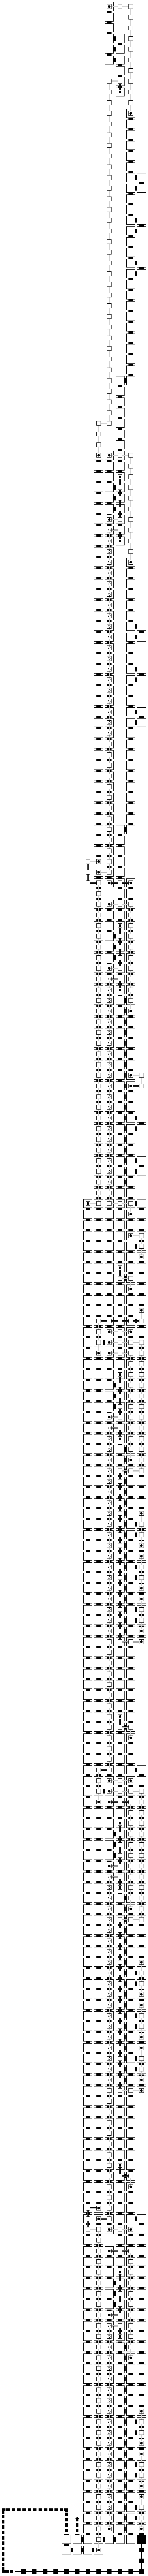
\includegraphics[width=0.45in]{overviews/general/cross_next_row}}}%
    ~
    \caption{\label{fig:crosser_gadgets} The {\tt Cross\_Next\_Row} gadget.}
\end{figure}
